\section{Konzept und Implementation}
\label{sec:Konzeption}
Folgend wird das entworfene Konzept, zur Lösung der unter \ref{cha:Aufgabenstellung} beschriebenen Aufgabenstellung, beschrieben. Es umfasst den Entwurf von konkreten Systemteilen und -Komponenten, die implementiert werden müssen. Weiter werden getroffene Entscheidungen zum Entwurf und zur Implementation der Komponenten beschrieben. Angetroffene Probleme werden vorgestellt und und deren Lösung erklärt\footnote{Konkrete technische Hindernisse mit Verweise auf Anhang zu Open Source changes/contributions oder auch technische Limitation wie bspw. go-ethereum mobile hat keine whisper API}.

Die Webapp ermöglicht es einem Owner, ein Objekt über einen in der Blockchain festgelegten Smart Contact zu vermieten. Er kann dabei das Depot und die Mietkosten festlegen. Ein Renter kann dann dieses Objekt für eine bestimmte Zeit mieten. Die Abwicklung des Vertrages und Begleichung der Kosten geschieht über die Auslösung durch den Renter in der Blockchain. Es gibt keinen Zwischenmann (z.B. Bank), der für die Überweisung zuständig ist, sondern das Geld fliesst vom Renter direkt zum Owner, basierend auf den definierten Regeln im Smart Contract.

Ein Objekt kann grundsätzlich alles sein: Ein elektrisches Fahrrad, eine Ferienwohnung oder ein Schließfach. Es muss jedoch möglich sein, einen Kontrollmechanismus anzubringen, der an eine Blockchain Node angebunden werden kann. Bei einem elektrischen Fahrrad wäre es z.B. möglich einen Minicomputer im Fahrgestellt zu montieren, welcher den Akku aktiviert oder deaktiviert und über eine Sim-Karte mit der Blockchain synchronisiert. Möchte ein Benutzer das Fahrrad verwenden, so müsste er dieses zuerst über die Blockchain mieten und erst dann kann er den Akku aktivieren. Die Mietkosten würden über den Smart Contract dem Anbieter des Fahrrades überwiesen werden.

\begin{figure}
\centering
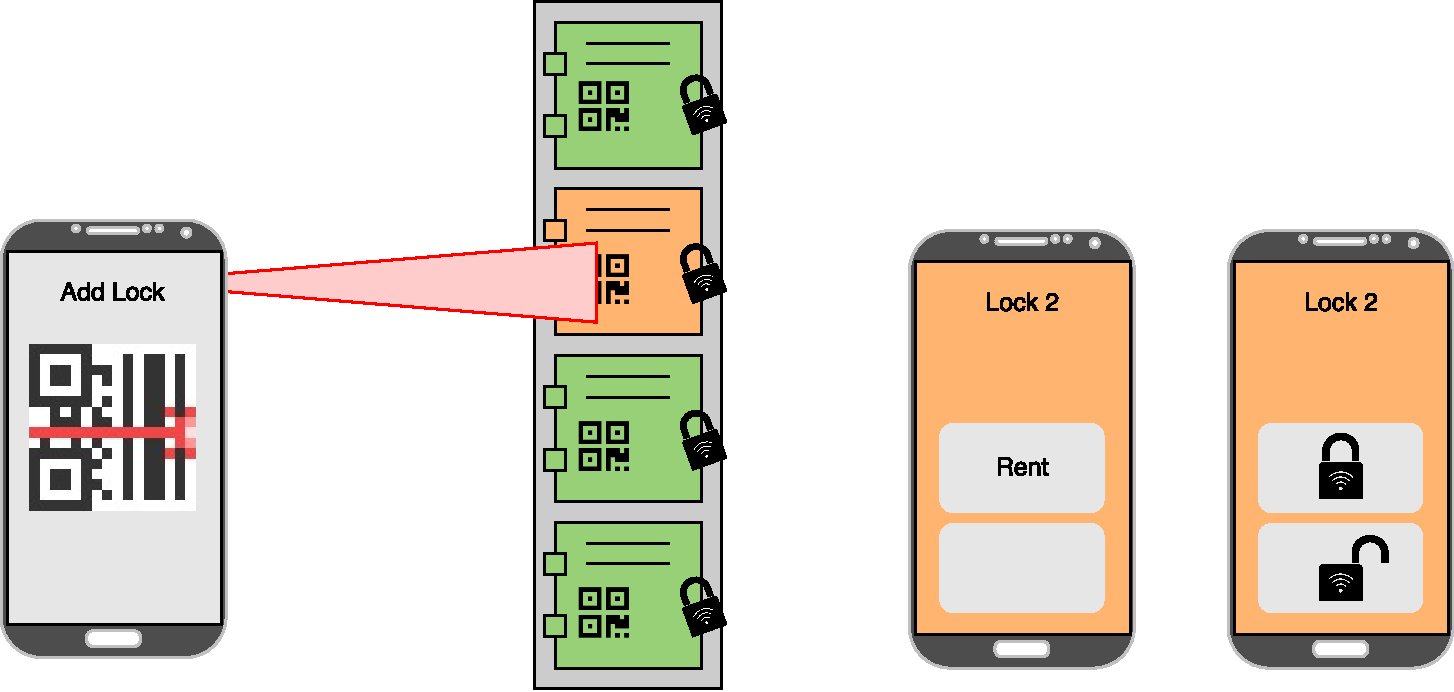
\includegraphics[width=.95\textwidth]{Mobile_Konzept}
\caption{Das Grobkonzept, dessen Umsetzung möglich ist}
\label{fig:Mobile_Konzept}
\end{figure}

\subsection{Sicherheit}
Im Design und bei der Umsetzung dieses Systems wurde angenommen, dass die Implementation des gesamten Ethereum Protokolls und der web3 Funktionen kryptographisch sicher ist und die Validität eines Smart Contracts nicht infrage gestellt werden kann, sofern die Blockchain in einem validen Zustand ist.\cite{github.com/ethereum/web3js, go-ethereum}

Der einzige selbst entwickelte Sicherheitskritische Aspekt ist bei der Übermittlung der Nachrichten mittels Whisper v5 (vgl. \ref{para:Whisper}). Entsprechend findet sich im Kapitel \ref{subsubsec:Sicherheitsaspekte} eine Abhandlung der gemachten Überlegungen und getroffene Massnahmen zur Sicherstellung der validen Herkunft der Nachrichten.

\subsection{Interaktion mit dem Demonstrator}
\label{sec:Interaktion mit dem Demonstrator}

Ein Benutzer muss sich zuerst als einen weiteren Node mit der Blockchain verbinden. Anschliessend kann er über die entwickelte Webapp (DAPP) mit dem System interagieren. 

\vspace{1em}\noindent
Folgende Interaktionen sind möglich.

\vspace{1em}\noindent
\textbf{Als Owner}
\begin{itemize}
    \item Neues Rentable erfassen
    \item Bestehende Rentable deaktivieren, aktivieren oder unbenutzbar machen
    \item Eigenschaften eines bestehenden Rentable ändern
    \item Rentable einem anderen Owner überschreiben
    \item Deposit von vergangenen Reservationen erhalten
\end{itemize}

\vspace{1em}\noindent
\textbf{Als potientieller Renter}
\begin{itemize}
    \item Informationen und Verfügbarkeit eines Rentables prüfen
    \item Ein Rentable reservieren (rent)
    \item Gutschriften abheben
\end{itemize}

\vspace{1em}\noindent
\textbf{Als aktueller Renter (current renter)}
\begin{itemize}
    \item Sperren und Entsperren des Rentables (Lock/Unlock)
    \item Zurückgeben des Schließfachs (Unclaim)
\end{itemize}

\subsection{Regeln}
\begin{enumerate}
    \item Es gibt keine Reservationsüberlappungen
\end{enumerate}

\subsection{Fallbeispiele}
\label{sec:Fallbeispiele}
Die folgenden Fallbeispiele erläutern das Zusammenspiel der Interaktionen und die Verschiebung der priviligierten Rechte entlang der Zeitachse.

\subsubsection{Normal-Fall}
In Abb.~\ref{fig:Cases}\,(a) reserviert Benutzer A das Schliessfach von $t_{R1}$ bis $t_{R2}$ zum Zeitpunkt $t_0$. Das Deposit und die Mietkosten werden ihm somit abgezogen.
Zum Zeitpunt $t_{R1}$ wird Benutzer A zum \emph{Current Renter} und besitzt dadurch privilegierten Zugriff. Er kann jetzt das Schliessfach öffnen (Unlock) und schliessen (Lock). Nach einer gewissen Zeit noch vor Ablauf der Reservation, entschliesst sich Benutzer A das Schliessfach wieder abzugeben (Unclaim), da er es nicht mehr benötigt. Die Reservation wird somit auf diesen Zeitpunkt gekürzt und Benutzer A erhählt sein Deposit und die Mietkosten für die ungenutzte Zeit zurück. Die priviligierten Rechte werden umgehend wieder an den Owner abgegeben.

\begin{figure}
\centering\small
\setlength{\tabcolsep}{0mm}	% alle Spaltenränder auf 0mm
\begin{tabular}{c@{\hspace{12mm}}c} % mittlerer Abstand = 12mm
  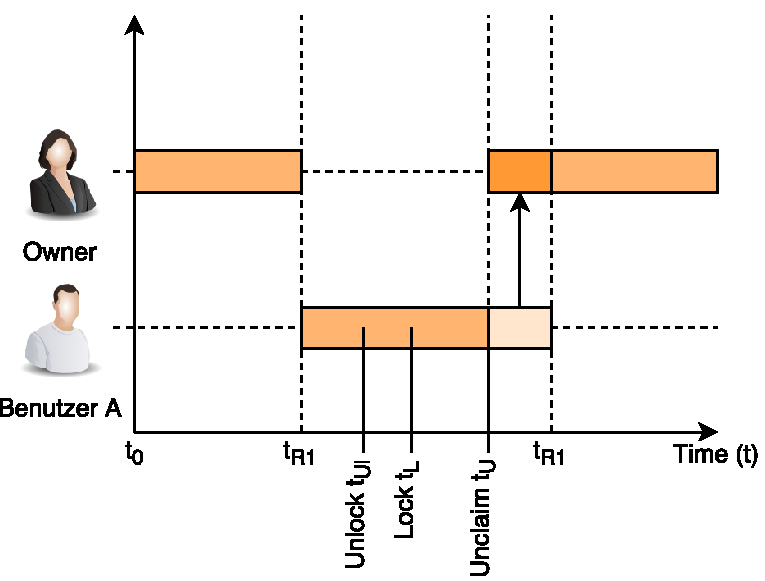
\includegraphics[width=.45\textwidth]{Case-Normal} &
  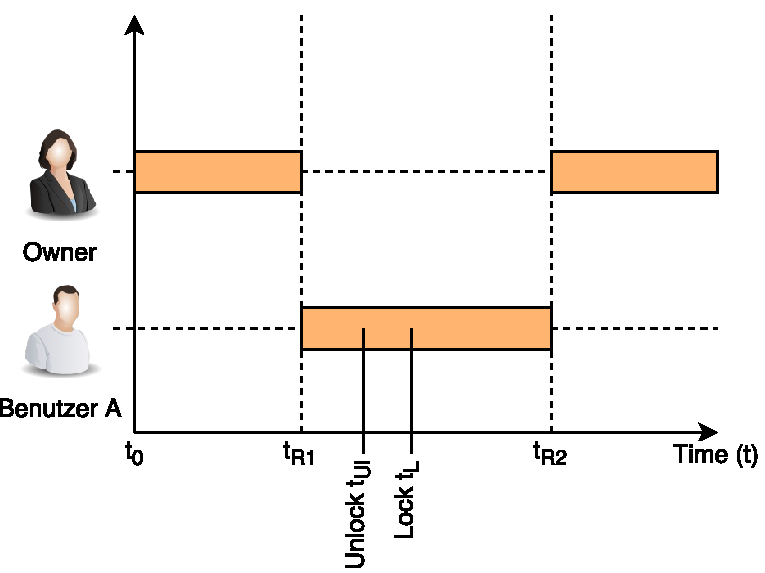
\includegraphics[width=.45\textwidth]{Case-No-Unclaim} \\
  (a) & (b) 
\end{tabular}
%
\caption{Verschiedene Fälle -- 
Normal-Fall (a), Keine-Rückgabe (b).}
\label{fig:Cases}
\end{figure}

%\begin{figure}
%\centering
%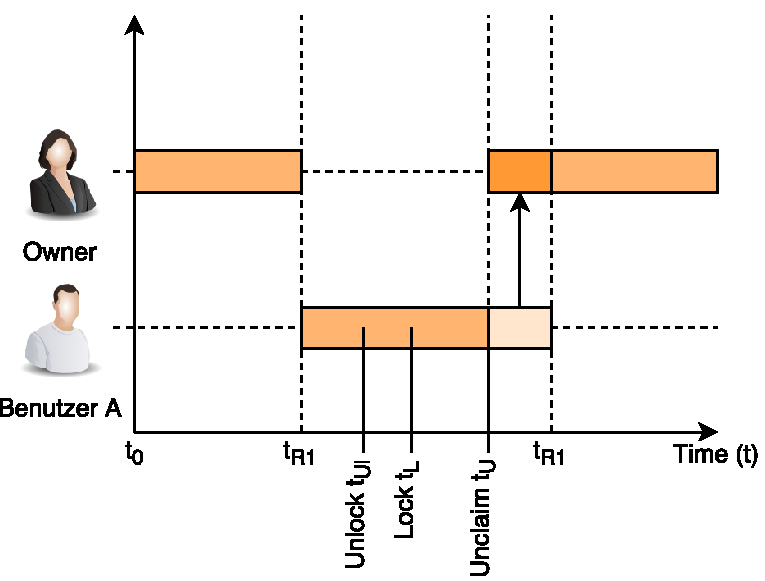
\includegraphics[width=.95\textwidth]{Case-Normal}
%\caption{Normal-Fall}
%\label{fig:Case-Normal}
%\end{figure}

\subsubsection{Reservationsende ohne Betätigung der Rückgabe}
Wie im Normal-Fall beschrieben, ist Benutzer A momentaner Renter (current renter) des Schliessfaches. Anstelle jedoch das Schließfach wieder zurückzugeben, lässt er die Reservationszeit auslaufen. Zum Zeitpunkt $t_{R2}$ werden ihm die Rechte entzogen und er erhält keine Rückerstattung des Deposits. Es liegt also in Benutzer A seinem Interesse, alle eingeschlossenen Gegestände vor Ablauf der Reservation aus dem Schließfach zu nehmen und dieses zurückzugeben (Unclaim). Siehe Abb.~\ref{fig:Cases}\,(b) als Illustration.

\subsubsection{Fall von Schäden}
Benutzer A reserviert wie im Normal-fall ein Schliessfach. Zum Zeitpunkt t1 will er das Schliessfach öffen (Unlock), dieses reagiert jedoch nicht. Er muss nun Kontakt mit dem Owner aufnehmen und die Sache klären. Auf jeden Fall sollte er nun das Schliessfach zurückgeben (Unclaim) um die Kosten niedrig zu halten, im Falle, dass sich der Owner nicht auffinden lässt oder dieser kein Interesse zeigt.

Im Rahmen dieser Arbeit wurde auch ein Konzept überlegt, wie solche Probleme vermindert werden könnten. Durch Einführen eines Review Systems, wo Benutzer die Owner beurteilen können. Owner mit einer guten Bewertung (Score) wären dann vertrauenswürdiger.
